\documentclass{report}

% ----------------------------------------------------
% PACKAGE
% ----------------------------------------------------

\usepackage{graphicx}
\usepackage{amsmath}
\usepackage{amsfonts}
\usepackage{amssymb}
\usepackage{hyperref}
\usepackage[a4paper, portrait, margin=0.75in]{geometry}
\usepackage[italian]{babel}
\usepackage{enumerate}% http://ctan.org/pkg/enumerate

\hypersetup{
    colorlinks=true,
    linkcolor=black,
    urlcolor=blue,
}

\title{Analisi dei dati \\[1ex] \large Un goliardico riassunto}
\author{Ollari Dmitri}

\begin{document}
    \maketitle
    

    \tableofcontents
    \listoffigures

    
\chapter{Introduzione alla statistica}


\section{Raccolta dati e statistica descittiva}
\begin{enumerate}
  \item Procedimento di raccolta dati
  \item Attenzione a come si compone il campione
  \item illustrare e sintetizzare i dati(statistica descittiva)
\end{enumerate}


\section{Inferenza statistica}
Mediante l'Inferenza statistica si possono predirre risultati mediante l'analisi dei dati.

\begin{enumerate}
  \item Tenere in conto il caso
  \item modello probabilistico(assunzioni sulla probabilit\`{a})
\end{enumerate}


\section{Popolazione e campioni}

Si vogliono risultati su gruppi estesi di persone, dove i vari sottogruppi devono essere 
rappresentati.

\textbf{Il campione \`{e} rappresentativo solo se \`{e} casuale.}


    
\chapter{Statistica descrittiva}

Permette la rappresentazione dei dati in maniera chiara, precisa, concisa e sintetica.

Si utilizzano diversi tipi di grafici in base al contesto.

\section{Grandezze per sintetizzare i dati}

Si hanno $n$ dati.

\begin{equation}
  n : x_1, x_2, \dots, x_n
\end{equation}

L'ampiezza(numerosit\`{a}) dei dati sar\`{a} $n$.
\subsection{Centro dei dati}
\subsubsection{Media campionaria}
La media campionaria \`{e} una media pesata!

\begin{equation}
    \bar{x} = \displaystyle\frac{1}{n} \displaystyle\sum_{i = 1}^{n} x_i
\end{equation}

Dove la $n$ rappresenta il numero di elementi presi in considerazione per la media.

\subsubsection{Mediana campionaria}

Avendo un insieme di dati $n$ \textbf{ordinato}:
\begin{itemize}
    \item Se $n$ è dispari, la mediana campionaria è il valore in posizione $(n + 1) / 2$
    \item Se $n$ è pari, la mediana campionaria è la media dei valori in posizione $n / 2$ e $n / 2 + 1$
\end{itemize}


\subsubsection{Varianza} 
Avendo un'insieme di dati $x_1, x_2, \dots, x_n$, la varianza campionaria è:

\begin{equation}
    s^2 = \displaystyle\frac{1}{n - 1} \displaystyle\sum_{i = 1}^{n} (x_i - \bar{x})^2
\end{equation}

\subsubsection{Devizione standard} 
Avendo un'insieme di dati $x_1, x_2, \dots, x_n$, la deviazione standard è:

\begin{equation}
    s = \sqrt{\displaystyle\frac{1}{n - 1} \displaystyle\sum_{i = 1}^{n} (x_i - \bar{x})^2}
\end{equation}


\subsection{Percentili campionari}

\begin{figure}[!ht]
    \begin{center}
        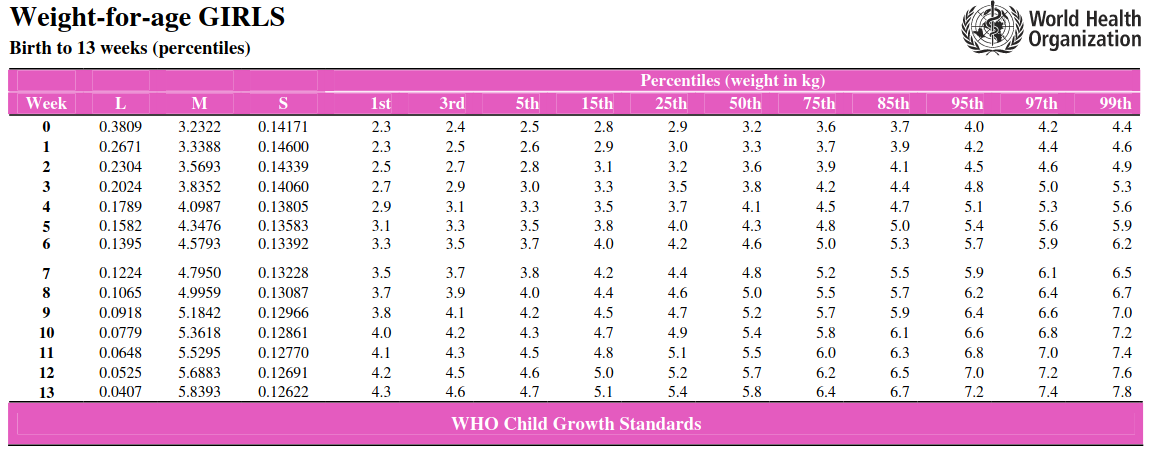
\includegraphics[width=0.8\textwidth]{./images/percentile_example.png}
    \end{center}
    \caption{Esempio percentili}
    \label{fig:esempio_percentili}
\end{figure}

Da questo graafico dell'OMS si capisce bene coasa sono i percentili. 

Le bambine che fanno parte del 25 esimo percentile hanno un peso alla nascita di $2.9$ Kg, 
il $25\%$ della bambine pesano meno e il $75\%$ delle bambine pesano di più. 

Il percentile divide i dati in due parti ben distinte, se il dato non è unico(due dati), si fa la media aritmetica. 

\subsubsection{Procedura}

Ho $n$ dati e voglio il valore del percentile k-esimo:
\begin{equation}
   p = \displaystyle\frac{k}{100} 
\end{equation}

\begin{equation}
   np = n \displaystyle\frac{k}{100} 
\end{equation}

Se $np$ non è intero, arrotondo al numero per eccesso successivo.



\subsubsection{Nota bene}
Sono quartili campionari: 
\begin{itemize}
    \item 25-esimo percentile
    \item 50-esimo percentile
    \item 75-esimo percentile
\end{itemize}

Notare che il 50-esimo percentile è la media campionaria.


\subsection{Box plot}
\begin{figure}[!ht]
    \begin{center}
        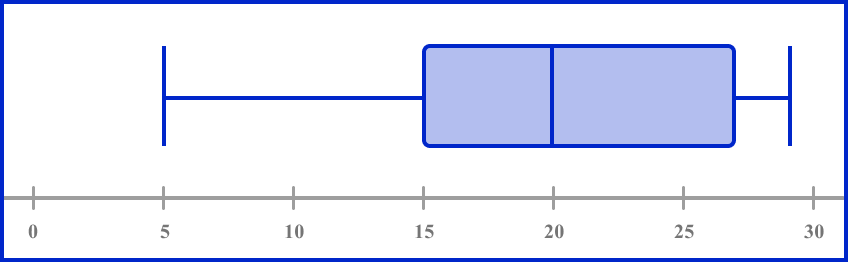
\includegraphics[width=0.5\textwidth]{./images/box_plot_example.png}
    \end{center}
    \caption{Esempio box plot}
    \label{fig:box_plot_example}
\end{figure}

Il disegno del box plot segue le seguenti regole:
\begin{itemize}
    \item linea da dato minore a dato maggiore
    \item box dal primo al terzo quartile
\end{itemize}

La lunghezza della linea rappresenta il campo di variazione(range dei valori), mentre la lunghezza del box 
rappresenta lo scarto interquartile. 

\section{Disuguaglianza di Chebyshev}
Avendo un'insieme di dati $x_1, x_2, \dots, x_n$ con media campionaria $\bar{x}$ e deviazione standard $s > 0$. 

Denoto con $S_k$ l'insieme degli indici dei dati compresi tra $\bar{x}-ks$ e $\bar{x}+ks$.

Essendo $\#S_k$ il numero di elementi dell'insieme $S_k$.(AKA cardinalità) 

Ne deriva la seguante equazione se $k \geq 0$:
\begin{equation}
   \displaystyle\frac{\#S_k}{n} \geq 1 - \displaystyle\frac{n - 1}{n k^2} > 1 - \displaystyle\frac{1}{k^2} 
\end{equation}


\section{Campioni normali}
Forma della distribuzione \textbf{caratteristica}:
\begin{itemize}
    \item a campana
    \item massimo sulla mediana
    \item simmetrica
\end{itemize}

Può essere approssimativamente normale o sbilanciata(skewed).


\subsection{Regola empirica}
\begin{itemize}
    \item Il $\sim 68\%$ dei dati si trova nella spazio $\bar{x} \pm s$
    \item Il $\sim 95\%$ dei dati si trova nella spazio $\bar{x} \pm 2s$
    \item Il $\sim 99.7\%$ dei dati si trova nella spazio $\bar{x} \pm 3s$
\end{itemize}


\section{Dati bivarianti}

Sono serie di dati diverrsi che hanno una correlazione fra di loro. 

La formula della correlazione è:
\begin{equation}
    (x_i - \bar{x})(y_i - \bar{y})
\end{equation}


Se il risultato è:
\begin{itemize}
    \item $> 0 \Rightarrow$ correlazione positiva
    \item $< 0 \Rightarrow$ correlazione negativa
\end{itemize}


\subsection{Coefficiente di correlazione campionaria}

\begin{equation}
   r = \displaystyle\frac{
        \displaystyle\sum_{i = 1}^{n} (x_i - \bar{x})(y_i - \bar{y})
   }{
        (n - 1)s_xs_y
   } 
\end{equation}


\begin{itemize}
    \item $r > 0 \Rightarrow$ correlazione positiva
    \item $r < 0 \Rightarrow$ correlazione negativa
\end{itemize}

\textbf{La correlazione è diversa dalla relazione di causa effetto.}



    \include{./2 - elementi di probabilità.tex}
    \chapter{Variabili aleatorie e valore atteso}

\section{Variabili aleatorie}

Con le variabili aleatorie si assegna la probabilit\`{a} ai valori possibili. 

Esempio dei due dadi: 
La probabilit\`{a} che il risultato della somma sia 3 si scrive cos\`{i}
\begin{equation}
   P(\{X = 3\}) = P\{(2,1),(1,2)\} 
\end{equation}

Quindi si hanno 2 casi favorevoli su 36 totali, che porta la probabilit\`{a} al valore di $0.055$. 

\section{Variabili aleatorie discrete e continue}

Le variabili aleatorie che prendono valori da insiemi finiti o numerabili prendono il nome di \textbf{discrete}. 

In alternativa le variabili non numerabili prendono il nome di \textbf{continue} e sono tutti quei valori 
che fanno parte dei numeri reali. 

\subsection{Funzione di ripartizione}

\begin{equation}
   F(x) = P(X \leq x) 
\end{equation}

La funzione $F(x)$ rappresenta la probabilit\`{a} con la quale la variabile aleatorie $X$ sia $\leq$ di $x$. 

La notazione $X \sim F$ indica che $F$ \`{e} la funzione di ripartizione di $X$. 

\subsection{Variabili aleatorie discrete e continue}
Se $X$ \`{e} una variabile aleatoria discreta, la sua \textbf{funzione id massa di probabilit\`{a}(PMF)} \`{e}: 
\begin{equation}
   p(a) = P(X=a) 
\end{equation}


\subsection{Funzioni di densit\`{a} di probabilit\`{a} di $X$(PDF)}

\begin{equation}
    1 = P(X \in \Re) = \displaystyle\int_{-\infty}^{+\infty} f(x)dx
\end{equation}

dove il limiti di integrazione sono dati dal range dei dati che stiamo considerando. 


ESEMPIO:
Variabile aleatoria $X$ con PDF:

\begin{equation}
    f(x) = \begin{cases}
        c(4x - 2x^2) \indent  0 < x < 2 \\
        0 \indent \indent \indent \indent else
    \end{cases}
\end{equation}

Per ottenere $c$:
\begin{equation}
    1 = c \displaystyle\int_{0}^{2} (4x - 2x^2)dx = c\Bigg[2x^2 - 2\displaystyle\frac{x^3}{3}\Bigg]_{x=0}^{x=2} = c \displaystyle\frac{8}{3}
\end{equation}
$c = \displaystyle\frac{3}{8}$

\section{Coppie di vettori di variabili aleatorie}


Utili a valutare la relazione tra variabili aleatorie. 

\subsection{Distribuzione congiunta per variabili aleatorie continue}


$X$ e $Y$ sono congiuntamente continue se esiste $f(x,y) > 0$ definita per tutti 
$x,y$ tale che ogni sottoinsieme $C$ del piano cartesiano sia:
\begin{equation}
   P((x, y) \in C) = \iint_{x,y \in C} f(x, y)dxdy
\end{equation}

Dove con $f(x, y)$ si intende la densit\`{a} congiunta. 


Facendo vari giri matematici si ottiene:
\begin{equation}
   \displaystyle\int_{b}^{b + db}\displaystyle\int_{a}^{a + da} f(x, y)dxdy \simeq f(a, b)dadb 
\end{equation}

\textbf{Vale solo se $da$ e $db$ sono molto piccoli e $f(a, b)$ \`{e} continua in $(a, b)$}. 


\subsection{Variabili aleatorie indipendenti}


\begin{equation}
   P(X \in A, Y \in B) = P(X \in A) P(Y \in B) 
\end{equation}

\subsection{Generalizzazione a pi\`{u} variabili aleatorie}

Ripartizione:
\begin{equation}
   F(a_1, a_2, \dots, a_n) = P(x_1 \leq a_1, \dots, x_n \leq a_n) 
\end{equation}

Se sono variabili discrete:
\begin{equation}
   p(x_1, x_2, \dots, x_n) = P(X_1 = x_1, X_2 = x_2, \dots, X_n = x_n) 
\end{equation}


Se sono continua devo usare le funzioni con gli integrali mega in sbatti. 

\subsection{Indipendenza}

Infinite variabili aleatorie sono indipendenti se ogni loro sottogruppo finito \`{e} formato da 
variabili aleatorie indipendenti. 

\textbf{mancano la densita condizionale e la distribuzioen condizionale}

\section{Valore atteso}

$X$ variabili aleatoria con valori $x_1, \dots$, il valore atteso di $X$:

\begin{equation}
   E[X] = \displaystyle\sum_{i} x_i P(X = x_i) 
\end{equation}

Il valore della sommatoria deve converge ad un numero inferiore a infinito. 

Praticamente la media pesata dei possibili valori di $X$, con pesi dati dalle probabilit\`{a}. 

$E[X]$ viene chaimata media di $X$ oppure aspettazione (expectation). 


\section{Proprietà del valore atteso}

Se $X$ è una variabile aleatoria discreta con funzione di massa di probabilità $p$, allora, per ogni 
funzione reale $g$:

\begin{equation}
    E[g(X)] = \displaystyle\sum_{x} g(x)p(x) 
\end{equation}


Se $X$ è una variabile aleatoria continua con funzione di densità di probabilità $f$, allora, per ogni 
funzione reale $g$:

\begin{equation}
    E[g(X)] = \displaystyle\int_{-\infty}^{+\infty} g(x)f(x)dx 
\end{equation}


\section{Variana}

Misura della variabilità della variabile aleatoria, la media $E[X]$ rappresenta il baricentro ma non 
è sufficiente. 

Sia $X$ una variabile aleatoria con media $\mu$, la varianza di $X$ si denota con $Var(X)$:
\begin{equation}
    Var(X) = E[(X-\mu)^2] 
\end{equation}


Però spesso viene più comoda la seguente formula:
\begin{equation}
    Var(X) = E[X^2] - E[X]^2 
\end{equation}




\subsection{Deviazione standard}
per calcolare la deviazioen standard basta:
\begin{equation}
    \sqrt{Var(X)} 
\end{equation}


\section{La covarianza e la varianza della somma di variabili aleatorie}

Avendo due variabili aleatorie $X$ e $Y$ con media $\mu_X$ e $\mu_Y$, la loro covarianza se esiste è:
\begin{equation}
    Cov(X, Y) = E[(X - \mu_X) (Y - \mu_Y)] 
\end{equation}


\textbf{Proprietà}
\begin{itemize}
    \item $Cov(X, Y) = Cov(Y, X)$ 
    \item $Cov(X, X) = Var(X)$ 
    \item $Cov(aX, Y) = a Cov(X, Y) = Cov(X, aY)$ 
\end{itemize}

\subsection{Coefficiente di correlazione lineare}

\begin{equation}
    Corr(X, Y) = \displaystyle\frac{Cov(X, Y)}{\sqrt{Var(X)Var(Y)}} 
\end{equation}

\section{La funzione generatrice dei momenti}





   


    
\end{document}
